\documentclass[a4paper,12pt]{article}
%%%%%%%%%%%%%%%%%%%%%%%%%%%%%%%%%%%%%%%%%%%%%%%%%%%%%%%%%%%%%%%%%%%%%%%%%%%%%%%%%%%%%%%%%%%%%%%%%%%%%%%%%%%%%%%%%%%%%%%%%%%%%%%%%%%%%%%%%%%%%%%%%%%%%%%%%%%%%%%%%%%%%%%%%%%%%%%%%%%%%%%%%%%%%%%%%%%%%%%%%%%%%%%%%%%%%%%%%%%%%%%%%%%%%%%%%%%%%%%%%%%%%%%%%%%%
\usepackage{eurosym}
\usepackage{vmargin}
\usepackage{amsmath}
\usepackage{graphics}
\usepackage{epsfig}
\usepackage{subfigure}
\usepackage{fancyhdr}
%\usepackage{listings}
\usepackage{framed}
\usepackage{graphicx}

\setcounter{MaxMatrixCols}{10}
%TCIDATA{OutputFilter=LATEX.DLL}
%TCIDATA{Version=5.00.0.2570}
%TCIDATA{<META NAME="SaveForMode" CONTENT="1">}
%TCIDATA{LastRevised=Wednesday, February 23, 2011 13:24:34}
%TCIDATA{<META NAME="GraphicsSave" CONTENT="32">}
%TCIDATA{Language=American English}

\pagestyle{fancy}
\setmarginsrb{20mm}{0mm}{20mm}{25mm}{12mm}{11mm}{0mm}{11mm}
\lhead{Dublin \texttt{R}} \rhead{10 April 2013}
\chead{Introduction to \texttt{R} (Module A)}
%\input{tcilatex}


\begin{document}

\tableofcontents
\newpage


\section{Review of Logistic Regression}
% http://www.nesug.org/proceedings/nesug06/an/da26.pdf
% http://www.ccsr.ac.uk/publications/teaching/blr.pdf
% http://www.southampton.ac.uk/ghp3/docs/unicef/presentation7.1a.pdf
% ftp://public.dhe.ibm.com/software/analytics/spss/documentation/statistics/20.0/en/client/Manuals/IBM_SPSS_Regression.pdf
% http://www.umass.edu/statdata/statdata/data/

%---------------------------------------------------------------%
\subsection{Generalized Linear Model}

The term �generalized linear model� is used to describe a procedure for
transforming the dependent variable so that the �right hand side� of the model
equation can be interpreted as a �linear combination� of the explanatory variables:

\[ \operatorname{F(y)} = b_0 + b_1x_1 + b_2x_2 + b_3x_3 \ldots b_kx_k + e \]

In situations where the dependent (y) variable is continuous and can be
reasonably assumed to have a normal distribution we do not transform the y
variable at all and we can simply run a multiple linear regression analysis.

Otherwise some sort of transformation is applied.
%---------------------------------------------------------------%
\subsection{Logistic Regression}
logistic regression or logit regression is a type of regression analysis used for predicting
the outcome of a categorical dependent variable (a dependent variable that can take on a limited number of values,
whose magnitudes are not meaningful but whose ordering of magnitudes may or may not be meaningful)
based on one or more predictor variables.



\begin{itemize}
\item[1.)] Logistic regression is intended for the modeling
of dichotomous categorical outcomes (e.g., characterized by binary responses: buy vs Don't buy, dead vs. alive, cancer vs. none,�).


\item[2.)] We want to predict the probability of a particular response  (0 to 1 scale).

\item[3.)] For binary responses, linear regression should not be used for several reasons
but the most common-sense reason is that linear regression can provide predictions NOT on a 0 to 1 scale.
but rather a predicted response of some numeric value (e.g 2.4 or -800.3).

\item[4.)] We need a way to link the probabilistic response variable to the continuous and/or categorical predictors and
keep things on this 0 to 1 scale.

\item[5.)] Logistic regression winds up transforming the probabilities to odds and then taking the natural logarithm of these odds, called logits.


\item[6.)] Suppose a response variable is passing a test (by convention, 0=no and 1=yes).
You have 1 predictor - number of days present in class over the past 30 days.
Suppose the regression coefficient (often just called beta) in the output is .14.
You would then say that, on average, as class presence increases by 1 day, the natural logarithm of the
odds of passing the test increases by .14.

\item[7.)] For the interpretation, you can just talk about the odds.
Most computer output will give you this number.
Suppose the answer in odds is 1.24. Then, you just say that,on average, as class presence increases by 1 day,
the odds of passing the test are multiplied by 1.24.
In other words, for each additional day present, the odds of passing are 24% greater than that of not passing.

\item[8.)] To validate our findings, normally, we test whether the regression coefficient is equal to zero in the population.
In logistic regression, the corresponding value for the odds is one (not zero). We got an odds of 1.24.
Can we trust this? Or should we go with one (which would mean that the odds are the same for both passing and not passing,
 and hence class presence makes no difference at all)?  Look at the p-value (significance). If it less than .05 (by convention), you have enough evidence to reject
the notion that the odds are really one. You go ahead and support the 1.24 result.
\end{itemize}


%-------------------------------------------%
\subsection{Odds}
The odds in favor of an event or a proposition are the ratio of the probability that an event will happen to the probability that it will not happen.
'Odds' are an expression of relative probabilities. Often 'odds' are quoted as odds against, rather than as odds in favor of, because of the possibility of confusion of the latter with the fractional probability of an event occurring.
\[ \operatorname{Odds} = \frac{p}{1-p} \]

\subsubsection{Example}
There are 5 pink marbles, 2 blue marbles, and 8 purple marbles.

\begin{itemize}
\item What is the probability of picking a blue marble? (Answer: 2/15).
\item What are the odds in favor of picking a blue marble? (Answer: 2/13).
\end{itemize}



%--------------------------------------------%
\subsection{Log-Odds}
As an alternative to modeling the value of the outcome, logistic regression focuses instead upon the
relative probability (odds) of obtaining a given result category. The natural logarithm of the odds is
linear across most of its range, allowing us to continue using many of the methods developed for linear models.
The result of this type of regression can be expressed as follows:
\[ \operatorname{Ln} \left[ \frac{p}{1-p} \right] = b_0 + b_1x_1 + b_2x_2 + b_3x_3 \ldots b_kx_k + e \]

%-------------------------------------------%
\subsection{Odds Ratio}
Suppose that in a sample of 100 men, 90 drank wine in the previous week, while in a sample of
100 women only 20 drank wine in the same period. The odds of a man drinking wine are 90 to 10,
or 9:1, while the odds of a
woman drinking wine are only 20 to 80, or 1:4 = 0.25:1. The odds ratio is thus 9/0.25, or 36,
showing that men are much more likely to drink wine than women. The detailed calculation is:
\[{ 0.9/0.1 \over 0.2/0.8}=\frac{\;0.9\times 0.8\;}{\;0.1\times 0.2\;} ={0.72 \over 0.02} = 36.\]
This example also shows how odds ratios are sometimes sensitive in stating relative positions:
in this sample men are 90/20 = 4.5 times more likely to have drunk wine than women, but have 36 times the odds.


\subsubsection{Confidence Intervals for Odds Ratios}
Many statistical implementations of logistic regression include Confidence Intervals for the odds ratios.
Odds ratios whose confidence limits exclude 1 are statistically significant.
The odds ratio is referred to in SPSS as \texttt{\textbf{Exp(B)}}, the exponentiation of the B coefficient
%-------------------------------------------%
\subsection{Odds Ratio Example}
These data are taken from the British Election Study 2005 pre-campaign and
post-election panel data. We will consider the propensity to vote (sometimes called ``turnout") as the
dependent variable, which has 2 categories. 0=did not turn out to vote, 1 turned
out to vote.
% \begin{center}
% \begin{figure}
%  % Requires \usepackage{graphicx}
%  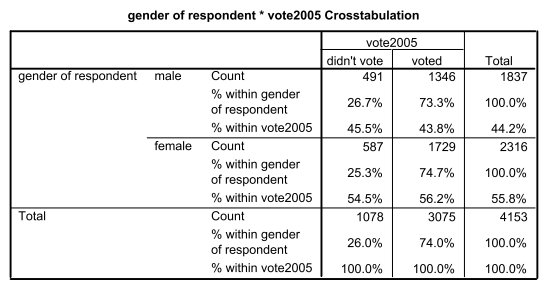
\includegraphics[scale=0.6]{images/LogWeek10A}\\
%  \caption{General Election 2005}
% \end{figure}
% \end{center}

% Image LogWeek10-A

The odds of a male turning out to vote are:
\[1346/491 = 2.741\]
The odds of female turning out to vote are
\[1729/587 = 2.945\]
The Odds ratio (female: male) are
(1729/587) / (1346/491) = 1.074

%-------------------------------------------%
\subsection{Logit}
The \textbf{logit} of a number $p$ between 0 and 1 is given by the formula:

\[\operatorname{logit}(p)=\log\left( \frac{p}{1-p} \right) =\log(p)-\log(1-p). \!\]

%-------------------------------------------%
\subsection{Logistic function}

The logistic function of any number is given by the inverse-logit:

\[\operatorname{logit}^{-1}(\alpha) = \frac{1}{1 + \operatorname{exp}(-\alpha)} = \frac{\operatorname{exp}(\alpha)}{1 + \operatorname{exp}(\alpha)}\]

%-------------------------------------------%


\subsection{Dummy variables}
When an explanatory variable is categorical we can use \textbf{dummy variables} to contrast
the different categories. For each variable we choose a baseline category and then
contrast all remaining categories with the base line. If an explanatory variable
has k categories, we need k-1 dummy variables to investigate all the differences in
the categories with respect to the dependent variable.

For example suppose the explanatory variable was \textbf{\textit{housing}} coded like this:
\begin{itemize}
\item[1:] Owner occupier
\item[2:] renting from a private landlord
\item[3:] renting from the local authority
\end{itemize}

We would therefore need to choose a baseline category and create two dummy
variables. For example if we chose owner occupier as the baseline category we
would code the dummy variables (House1 and House2) like this

%Tenure: &House1 &House2\\
%Owner occupier &0& 0\\
%Rented private &1 &0\\
%Rented local authority &0 &1\\

\subsection{Log Likelihood}
A ``likelihood" is a probability, specifically the probability that the observed values of the dependent may be predicted from the observed values of the independents. 

Like any probability, the likelihood varies from 0 to 1. The log likelihood (LL) is its log and varies from 0 to minus infinity (it is negative because the log of any number less than 1 is negative). LL is calculated through iteration, using maximum likelihood estimation (MLE).


\subsection{Maximum Likelihood Estimation}
Maximum likelihood estimation, MLE, is the method used to calculate the logit coefficients. This contrasts to the use of ordinary least squares (OLS) estimation of coefficients in regression. OLS seeks to minimize the sum of squared distances of the data points to the regression line. MLE seeks to maximize the log likelihood, LL, which reflects how likely it is (the odds) that the observed values of the dependent may be predicted from the observed values of the independents. (Equivalently MLE seeks to minimize the -2LL value.)

MLE is an iterative algorithm which starts with an initial arbitrary ``guesstimate" of what the logit coefficients should be, the MLE algorithm determines the direction and size change in the logit coefficients which will increase LL. After this initial function is estimated, the residuals are tested and a re-estimate is made with an improved function, and the process is repeated (usually about a half-dozen times) until convergence is reached (that is, until LL does not change significantly). There are several alternative convergence criteria.
%-------------------------------------------%

\subsection{Wald statistic}
he Wald statistic is commonly used to test the significance of individual logistic regression coefficients for each independent variable (that is, to test the null hypothesis in logistic regression that a particular logit (effect) coefficient is zero). 

The Wald Statistic is the ratio of the unstandardized logit coefficient to its standard error. The Wald statistic and its corresponding p probability level is part of SPSS output in the section \textbf{\textit{Variables in the Equation.}} This corresponds to significance testing of b coefficients in OLS regression. The researcher may well want to drop independents from the model when their effect is not significant by the Wald statistic.
\newpage
\subsection{SPSS Output}
The variable Vote2005 is a binary variable describing turnout at a general election. The predictor variables are gender and age.
\begin{center}
\begin{figure}[h!]
  % Requires \usepackage{graphicx}
  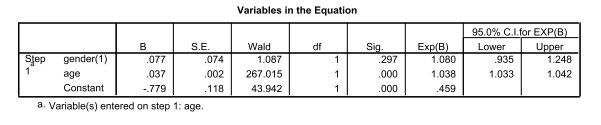
\includegraphics[scale=0.6]{images/LogWeek10B.jpg}\\
  \caption{General Election 2005}
\end{figure}
\end{center}

% Image LogWeek10-B

\[\mbox{logit(vote2005)} = -.779 + .077\mbox{gender(1)}+.037\mbox{age}\]

The age coefficient is statistically significant. Exp(B) for age is 1.038, which
means for each year different in age, the person is 1.038 times more likely to turn
out to vote, having allowed for gender in the model. Eg. a 21 year old is 1.038
times as likely to turn out to vote than a 20 year old. This might not seem much
of a difference but a 20 year difference leads to a person being $1.038^20 = 2.11$
times more likely to turn out to vote. E.g. a 40 year old is 2.11 times more likely to
turn out to vote than a 20 year old, having allowed for gender in the model.


The gender coefficient is not statistically significant.


%-------------------------------------------%
\subsection{Hosmer-Lemeshow Goodness-of-Fit}
The Hosmer-Lemeshow Goodness-of-Fit
test tells us whether we have constructed a valid overall model or not.
If the model is a good fit to the data then the HosmerLemeshow Goodness-of-Fit test should have an associated p-value greater than 0.05.


%-------------------------------------------------------%
\subsection{Pseudo R-squares}
Cox \& Snell R Square and Nagelkerke R Square are two measures from the \textbf{pseudo R-squares} family of measures.

Logistic regression does not have an equivalent to the R-squared that is found in OLS regression; however, many researcehrs have tried to come up with one.  There are a wide variety of pseudo-R-square statistics.  

Because this statistic does not mean what R-squared means in OLS regression (the proportion of variance explained by the predictors), we suggest interpreting this statistic with great caution.

\subsubsection{Cox \& Snell R Square}
Cox and Snell's R-Square is an attempt to imitate the interpretation of multiple R-Square based on the likelihood, but its maximum can be (and usually is) less than 1.0, making it difficult to interpret. It is part of SPSS output.

\subsubsection{Nagelkerke's R-Square}
Nagelkerke's R-Square is a further modification of the Cox and Snell coefficient to assure that it can vary from 0 to 1. Nagelkerke's R-Square will normally be higher than the Cox and Snell measure. It is part of SPSS output and is the most-reported of the R-squared estimates.
\newpage
\subsection{HSB2 Example}
The hsb2 dataset is taken from a national survey of high school seniors. Two hundred observation were randomly sampled from the High School and Beyond survey. Descriptive statistics and exploratory data analysis are shown below.
Because we do not have a suitable dichotomous variable to use as our dependent variable, we will create one (which we will call honcomp, for honors composition) based on the continuous variable write.  We do not advocate making dichotomous variables out of continuous variables; rather, we do this here only for purposes of this illustration.


Here is the list of variables in the file.
\begin{verbatim}

  obs:           200    highschool and beyond (200 cases)
 vars:            12    28 Feb 2005 09:25
-----------------------------------------------------------------------------
              variable
variable name   type   about the variable
-----------------------------------------------------------------------------
id              scale  student id
female        nominal  (0/1)
race          nominal  ethnicity (1=hispanic 2=asian 3=african-amer 4=white)
ses           ordinal  (1=low 2=middle 3=high)
schtyp        nominal  type of school (1=public 2=private)
prog          nominal  type of program (1=general 2=academic 3=vocational)
read            scale  standardized reading score
write           scale  standardized writing score
math            scale  standardized math score
science         scale  standardized science score
socst           scale  standardized social studies score
hon           nominal  honors english (0/1)
\end{verbatim}
\newpage
\subsection{Hosmer-Lemeshow Prostate Example}
We will now consider a real life example to demonstrate Logistic Regression. This example is taken from a Prostate Cancer Study from Hosmer and Lemeshow (2000). The goal of the analysis is to determine if variables
measured at baseline can predict whether a tumour has penetrated the prostatic capsule. The variables are as follows:
\begin{center}
\begin{figure}[h!]
  % Requires \usepackage{graphicx}
  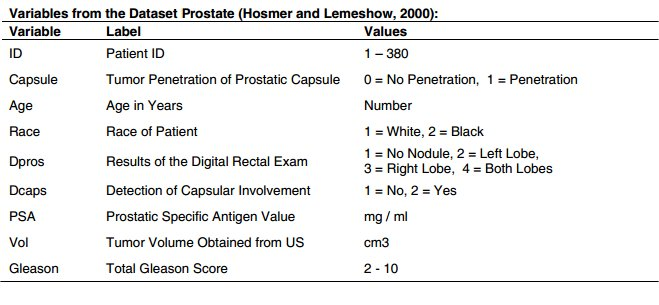
\includegraphics[scale=0.6]{images/LogWeek10C.jpg}\\
  \caption{Variables}
\end{figure}
\end{center}
\subsection{Kasser and Bruce Infarction Data Example}
We use a set of coronary data (Kasser and Bruce, 1969;
Kronmal and Tarter, 1974) to see if age, history of angina pectoris (ANGINA:
yes, no), history of high blood pressure (HIGHBP: yes, no), and functional class
(FUNCTION: none, minimal, moderate, and more than moderate) can be used to
predict the probability of past myocardial infarction (INFARCT: yes, no).



\subsection{The Likelihood Ratio Test}
The likelihood ratio test to test this hypothesis is based on the likelihood
function. We can formally test to see whether inclusion of an explanatory variable in a model tells us
more about the outcome variable than a model that does not include that variable. Suppose
we have to evaluate two models. 

\begin{center}
\begin{figure}[h!]
  % Requires \usepackage{graphicx}
  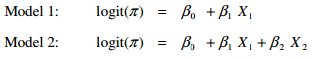
\includegraphics[scale=0.6]{images/LogWeek10D}\\
  \caption{Variables}
\end{figure}
\end{center}
Here, Model 1 is said to be nested within Model 2 � all the explanatory variables in Model 1
(X1) are included in Model 2. We are interested in whether the additional explanatory
variable in Model 2 ($X_2$) is required, i.e. does the simpler model (Model 1) fit the data just as
well as the fuller model (Model 2). In other words, we test the null hypothesis that $\beta_2 = 0$
against the alternative hypothesis that $\beta_2 \neq 0$. 

\subsection{Multinomial Logistic Regression}
Multinomial Logistic Regression is useful for situations in which you want to be able to classify
subjects based on values of a set of predictor variables. This type of regression is similar to logistic
regression, but it is more general because the dependent variable is not restricted to two categories.
For Example, In order to market films more effectively, movie studios want to predict what type of
film a moviegoer is likely to see. By performing a Multinomial Logistic Regression, the studio
can determine the strength of influence a person�s age, gender, and dating status has upon the type
of film they prefer. The studio can then slant the advertising campaign of a particular movie
toward a group of people likely to go see it.
%-------------------------------------------------------------------------------------%
\newpage
\section{Stepwise Logistic Selection}
Stepwise logistic regression involves the stepwise (or one-by-one) selection of variables,
providing a fast and effective method to screen a large number of variables, and to fit
multiple logistic regression equations simultaneously.

In stepwise selection, an attempt is made to remove any insignificant variables from the model before adding a significant variable to the model.

Stepwise binary logistic regression is very similar to stepwise multiple regression in terms of its advantages and disadvantages. Stepwise logistic regression is designed to find the \textbf{\textit{most parsimonious}} set of predictors that are most effective in predicting the dependent variable.

\subsection{Procedure for Stepwise Selection}
Variables are added to the logistic regression equation one at a time, using the statistical criterion of reducing the \textbf{\textit{-2 Log Likelihood error}} for the included variables. (Recall: The lower the -2LL value, the better the fit of the model).

After each variable is entered, each of the included variables are tested to see if the model would be better off the variable were excluded. This does not happen often.

The process of adding more variables stops when all of the available variables have been included or when it is not possible to make a statistically significant reduction in -2 Log Likelihood using any of the variables not yet included.

Categorical variables are added to the logistic regression as a group. It is possible, and often likely, that not all of the individual dummy-coded variables will have a statistically significant individual relationship with the dependent variable. 
%We limit our interpretation to the dummy-coded variables that do have a statistically significant individual relationship.
\subsection{SPSS Implementation}
SPSS provides a table of variables included in the analysis and a table of variables excluded from the analysis.  It is possible that none of the variables will be included.  It is possible that all of the variables will be included.

The order of entry of the variables can be used as a measure of relative importance.

Once a variable is included, its interpretation in stepwise logistic regression is the same as it would be using other methods for including variables.
%-------------------------------------------------------%
\subsection{Advantages and Disadvantages}
Stepwise logistic regression can be used when the goal is to produce a predictive model that is parsimonious and accurate because it excludes variables that do not contribute to explaining differences in the dependent variable.

Stepwise logistic regression is less useful for testing hypotheses about statistical relationships. Its usage is recommended only for exploratory purposes, rather that as a formal procedure.

Stepwise logistic regression can be useful in finding relationships that have not been tested before. Its findings invite one to speculate on why an unusual relationship makes sense.

It is not legitimate to do a stepwise logistic regression and present the results as though one were testing a hypothesis that included the variables found to be significant in the stepwise logistic regression.

Using statistical criteria to determine relationships is vulnerable to over-fitting the data set used to develop the model at the expense of generalisability.

\begin{quote}
Menard (1995: 54) writes, "there appears to be general agreement that the use of computer-controlled stepwise procedures to select variables is inappropriate for theory testing because it capitalizes on random variations in the data and produces results that tend to be idosyncratic and difficult to replicate in any sample other than the sample in which they were originally obtained."
\end{quote}
%-------------------------------------------------------%
\subsection{Forward Selection}
You can estimate models using block entry of variables or any of the following stepwise
methods: forward conditional, forward LR, forward Wald, backward conditional, backward
LR, or backward Wald.


Forward selection is the usual option for a stepwise regression,
starting with the constant-only model and adding variables one at a time. The forward
stepwise logistic regression method utilizes the likelihood ratio test which tests the change in �2LL between steps to determine automatically which variables to add or drop from the model.

Method selection allows you to specify how independent variables are entered into the analysis.
Using different methods, you can construct a variety of regression models from the same set of
variables.

\begin{itemize}
\item[1] Enter. A procedure for variable selection in which all variables in a block are entered in a
single step.
\item[2] Forward Selection (Conditional). Stepwise selection method with entry testing based on
the significance of the score statistic, and removal testing based on the probability of a
likelihood-ratio statistic based on conditional parameter estimates.
\item[3] Forward Selection (Likelihood Ratio). Stepwise selection method with entry testing based
on the significance of the score statistic, and removal testing based on the probability of a
likelihood-ratio statistic based on the maximum partial likelihood estimates.  (LR stands for Likelihood Ratio and  is considered the criterion least prone to error.)
\item[4] Forward Selection (Wald). Stepwise selection method with entry testing based on the
significance of the score statistic, and removal testing based on the probability of the Wald
statistic.
\item[5] Backward Elimination (Conditional). Backward stepwise selection. Removal testing is based on
the probability of the likelihood-ratio statistic based on conditional parameter estimates.
\item[6] Backward Elimination (Likelihood Ratio). Backward stepwise selection. Removal testing
is based on the probability of the likelihood-ratio statistic based on the maximum partial
likelihood estimates.
\item[7] Backward Elimination (Wald). Backward stepwise selection. Removal testing is based on the
probability of the Wald statistic.
\end{itemize}
%-------------------------------------------------------%
\subsection{Cross Validation of Stepwise Regression}
When stepwise logistic regression is used, some form of validation analysis is a necessity. We will use 75/25\% cross-validation.

To do cross validation, we randomly split the data set into a 75\% training sample and a 25\% validation sample. We will use the training sample to develop the model, and we test its effectiveness on the validation sample to test the applicability of the model to cases not used to develop it.

In order to be successful, the follow two questions must be answers affirmatively:
Did the stepwise logistic regression of the training sample produce the same subset of predictors produced by the regression model of the full data set?

If yes, compare the classification accuracy rate for the 25\% validation sample to the classification accuracy rate for the 75\% training sample. If the \textbf{shrinkage} (accuracy for the 75\% training sample - accuracy for the 25\% validation sample) is 2\% (0.02) or less, we conclude that validation was successful.

Note: shrinkage may be a negative value, indicating that the accuracy rate for the validation sample is larger than the accuracy rate for the training sample. Negative shrinkage (increase in accuracy) is evidence of a successful validation analysis.

If the validation is successful, we base our interpretation on the model that included all cases.

%\subsection{Model Selection}
%Model selection is a fundamental task in data analysis,
%widely recognized as central to good inference. In many types of statistical software we have 4 automatic model
%selection techniques: forward selection, backward
%elimination, stepwise selection which combines the
%elements of the previous two, and the best subset
%selection procedure. The first three methods are based
%on the same ideas and we will talk only about stepwise
%selection as more flexible and sophisticated selection
%procedure. This choice is subjective, some researchers
%prefer to work with backward selection.
\end{document}
